%%%%%%%%%%%%%%%%%%%%%%%%%%%%%%%%%%%%%%%%%
% Beamer Presentation
% LaTeX Template
% Version 1.0 (10/11/12)
%
% This template has been downloaded from:
% http://www.LaTeXTemplates.com
%
% License:
% CC BY-NC-SA 3.0 (http://creativecommons.org/licenses/by-nc-sa/3.0/)
%
%%%%%%%%%%%%%%%%%%%%%%%%%%%%%%%%%%%%%%%%%

%----------------------------------------------------------------------------------------
%	PACKAGES AND THEMES
%----------------------------------------------------------------------------------------

\documentclass{beamer}
\usepackage{pgfpages}
\usepackage{colortbl}
\usepackage{booktabs}
\usepackage{multirow}
\usepackage[backend=bibtex, style=authoryear]{biblatex}
\addbibresource{U:/Literature/Databases/DTWrefs}
\AtBeginBibliography{\tiny}
\renewcommand{\footnotesize}{\tiny}
%\pgfpagesuselayout{4 on 1}[a4paper,border shrink=5mm, landscape]

\mode<presentation> {

% The Beamer class comes with a number of default slide themes
% which change the colors and layouts of slides. Below this is a list
% of all the themes, uncomment each in turn to see what they look like.

%\usetheme{default}
%\usetheme{AnnArbor}
%\usetheme{Antibes}
%\usetheme{Bergen}
%\usetheme{Berkeley}
%\usetheme{Berlin}
%\usetheme{Boadilla}
%\usetheme{CambridgeUS}
%\usetheme{Copenhagen}
%\usetheme{Darmstadt}
%\usetheme{Dresden}
%\usetheme{Frankfurt}
%\usetheme{Goettingen}
%\usetheme{Hannover}
%\usetheme{Ilmenau}
%\usetheme{JuanLesPins}
%\usetheme{Luebeck}
%\usetheme{Madrid}
%\usetheme{Malmoe}
%\usetheme{Marburg}
%\usetheme{Montpellier}
%\usetheme{PaloAlto}
%\usetheme{Pittsburgh}
%\usetheme{Rochester}
%\usetheme{Singapore}
%\usetheme{Szeged}
\usetheme{Warsaw}

% As well as themes, the Beamer class has a number of color themes
% for any slide theme. Uncomment each of these in turn to see how it
% changes the colors of your current slide theme.

%\usecolortheme{albatross}
%\usecolortheme{beaver}
%\usecolortheme{beetle}
%\usecolortheme{crane}
%\usecolortheme{dolphin}
%\usecolortheme{dove}
%\usecolortheme{fly}
%\usecolortheme{lily}
%\usecolortheme{orchid}
%\usecolortheme{rose}
%\usecolortheme{seagull}
\usecolortheme{seahorse}
%\usecolortheme{spruce}
%\usecolortheme{whale}
%\usecolortheme{wolverine}

%\setbeamertemplate{footline} % To remove the footer line in all slides uncomment this line
%\setbeamertemplate{footline}[page number] % To replace the footer line in all slides with a simple slide count uncomment this line

%\setbeamertemplate{navigation symbols}{} % To remove the navigation symbols from the bottom of all slides uncomment this line
}

\usepackage{graphicx} % Allows including images
\usepackage{booktabs} % Allows the use of \toprule, \midrule and \bottomrule in tables
\usepackage{array}
\usepackage{xcolor}
\usepackage{tabu}
\usepackage{textpos}
\usepackage{animate}
\usepackage{hyperref}
\usepackage{bm}

\pdfpageattr {/Group << /S /Transparency /I true /CS /DeviceRGB>>}
\definecolor{links}{HTML}{2A1B81}
\hypersetup{colorlinks,linkcolor=,urlcolor=links}

\addtobeamertemplate{frametitle}{}{%
\begin{textblock*}{100mm}(.9\textwidth,-0.75cm)
\includegraphics[height=0.7cm, trim=0cm 3.9cm 0cm 0cm, clip=true]{U:/Misc/Logos/LICTR_logo}
\end{textblock*}}



%----------------------------------------------------------------------------------------
% Presentation for RSS meeting, 30 mins, covering SMMR paper
%----------------------------------------------------------------------------------------

%----------------------------------------------------------------------------------------
%	TITLE PAGE
%----------------------------------------------------------------------------------------

\title{MDG: Decision-theoretic analysis of pilot trials} 

\author{Duncan T. Wilson}
\institute[LICTR] % Your institution as it will appear on the bottom of every slide, may be shorthand to save space
{
\includegraphics[height=0.7cm, trim=0cm 3.9cm 0cm 0cm, clip=true]{U:/Misc/Logos/LICTR_logo}\\
Clinical Trials Research Unit \\ % Your institution for the title page
Leeds Institute of Clinical Trials Research \\
University of Leeds \\
\medskip
\textit{d.t.wilson@leeds.ac.uk} % Your email address
}
\date{7th March 2018}


\begin{document}

\begin{frame}
\titlepage % Print the title page as the first slide
\end{frame}

%\begin{frame}
%\frametitle{Overview}
%\tableofcontents 
%\end{frame}

%\section{Background}

\begin{frame}
\frametitle{Fellowship}
\centering
Developing methods to design and analyse pilot trials of complex interventions, considering\ldots
\begin{itemize}
\item Frequentist methods (extending phase II designs, known nuisance parameters, multivariate testing);
\item Bayesian methods (unconditional probabilities of hypotheses, uncertainty in parameters);
\item Decision-theoretic methods (specifying a utility function, modelling the confirmatory RCT).
\end{itemize}
\end{frame}

\begin{frame}
\frametitle{Previously\ldots}
Last time I spoke at an MDG we discussed how a Bayesian approach can help us handle uncertainty in, e.g., an ICC $\rho$ of a cluster trial:
\begin{align*}
n &= n_{i}[1+(m-1)\rho] \\
n_{i} &= \text{sample size required when clustering is ignored}
\end{align*}

Defining a (subjective prior) of $\rho \sim Beta(4, 58)$ (say), will give a posterior after seeing the pilot data.
\end{frame}

\begin{frame}
\frametitle{Uncertainty}
\vspace{3mm}
\centering
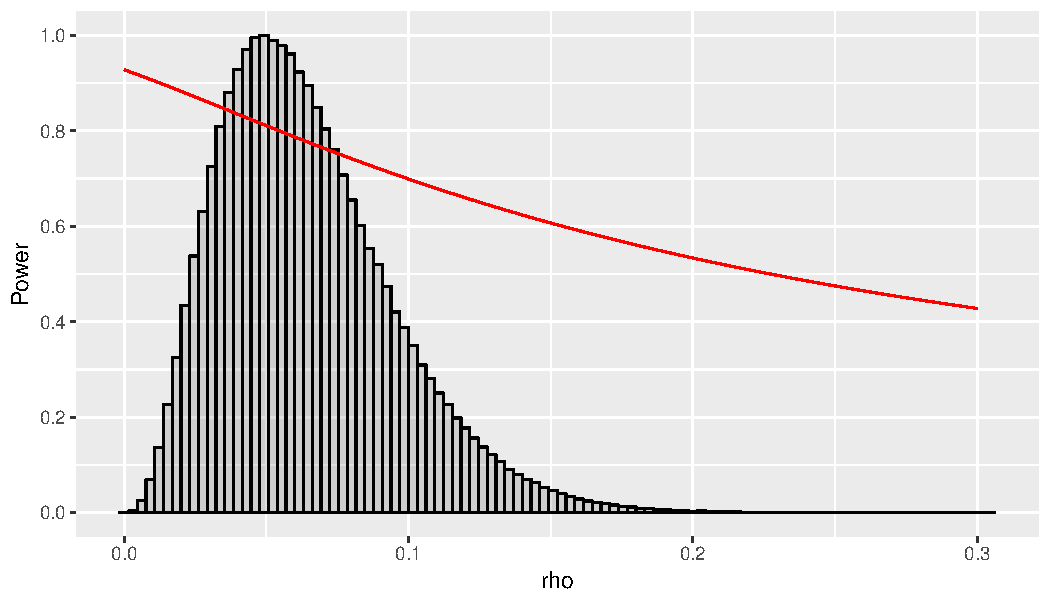
\includegraphics[scale=0.45]{prior_ICC}
\end{frame}

\begin{frame}
\frametitle{Uncertainty}
Uncertainty about $\rho$ propagates to uncertainty about power for fixed $n$:\\
\vspace{3mm}
\centering
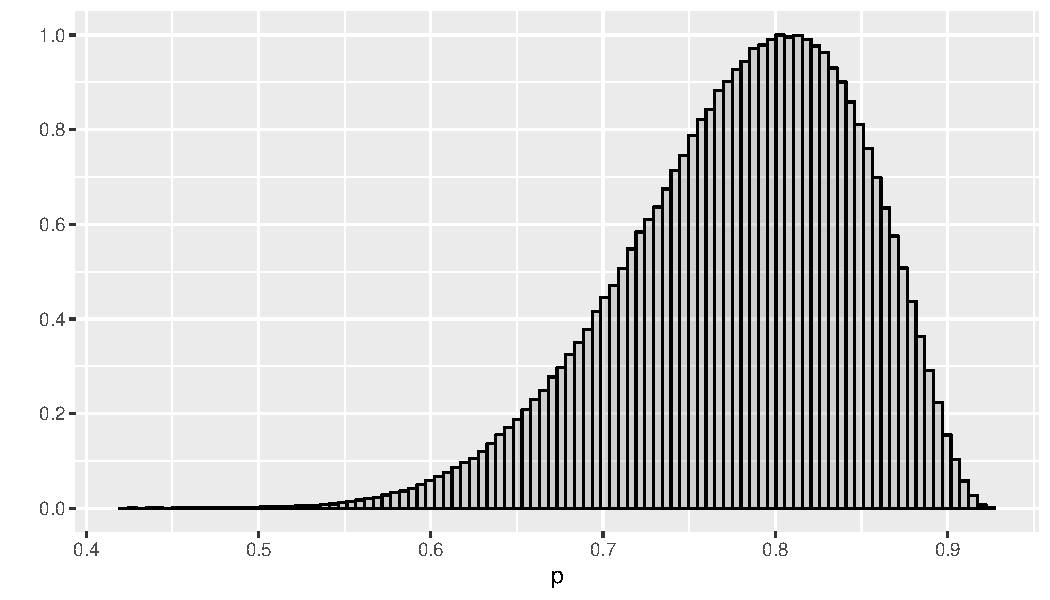
\includegraphics[scale=0.45]{prior_power}
\end{frame}


\begin{frame}
\frametitle{Assurance}
Focussed on methods of assurance - calculating the unconditional probability of an event. Most commonly, the rejection of the null in a freq. test, denoted $A$:
\begin{align*}
\text{assurance} = Pr[A] &= \int Pr[A \mid \theta]p(\theta) d\theta \\
 p(\theta) &= \text{probability density function of } \theta
\end{align*}

(Other types of events considered too, e.g. rejecting the null \emph{and} the true effect is meaningful)
\end{frame}

\begin{frame}
\frametitle{Utility}
Although assurance is arguably easier to interpret than conditional power, it isn't clear how to balance it against type I error and sample size costs when designing a trial. Alternative:

\begin{itemize}
\item Specify a utility function $u(d, \theta)$ ($d = $ trial design)
\item{ We can then choose the design which maximises the expected utility:
	\begin{equation}
	\arg\max_{d} ~ \mathbb{E}_{\theta}[u(d, \theta)]
	\end{equation}}
\item We will parametrise the design by $d = (\alpha, n)$, the type I error rate and the sample size.
\end{itemize}
\end{frame}

\begin{frame}
\frametitle{Maximising expected utility}
Why might we want to use a decision-theoretic approach? Axioms:

\begin{enumerate}
\item The relation $\succeq$, where $c_{1} \succeq c_{2}$ means $c_{1}$ is at least as good as $c_{2}$, is a weak ordering (i.e. complete and transitive) on $\mathcal{C}$, the space of consequences.
\item There exists $c^{*}, c_{*} \in \mathcal{C}$ such that $c^{*} \succ c_{*}$ and $\forall c \in \mathcal{C}, c^{*} \succeq c \succeq c_{*}$.
\item \ldots
\end{enumerate}

Axioms imply that there exists a $u: \mathcal{C} \rightarrow \mathbb{R}$ such that $\forall c_{1}, c_{2} \in \mathcal{C}$:
\begin{equation}
c_{1} \succeq c_{2} \Leftrightarrow u(c_{1}) \geq u(c_{2})
\end{equation}
\end{frame}

\begin{frame}
\frametitle{Scope for today}
We will consider:
\begin{itemize}
\item A pilot trial has been conducted;
\item We have a (empirical or mathematical) posterior distribution on the unknown treatment difference $\theta$;
\item A `confirmatory' balanced parallel group RCT is to be designed, i.e. $d = (\alpha, n)$ is to be chosen;
\item The primary endpoint and corresponding statistical test have been selected;
\end{itemize}
What designs are admissible? How do we choose the optimum?
\end{frame}

\begin{frame}
\frametitle{A single-attribute value function}
We have two attributes to the problem - the efficacy $\theta$ (benefit), and the sample size $n$ (cost). We assume these are \emph{preferentially independent}:
\begin{align}
& (\theta, n') \succeq (\theta', n') \\
\Rightarrow  & (\theta, n) \succeq (\theta', n) ~ \forall ~ n
\end{align}
We then focus on defining a single-attribute \emph{value} function $v(a, \theta)$, where $a$ is the action taken as a result of the test - stop $(-)$ or go $(+)$.
\end{frame}

\begin{frame}
\frametitle{A single-attribute value function}
\begin{align}
v(+, \theta) = \theta  \\
v(-, \theta) = 0
\end{align}
\end{frame}

\begin{frame}
\frametitle{A single-attribute value function}
Center at $\theta^{*}$, the \emph{minimal clinically important difference}:
\begin{align}
v(+, \theta) = \theta - \theta^{*} \\
v(-, \theta) = 0
\end{align}
\end{frame}

\begin{frame}
\frametitle{A single-attribute value function}
Account for the \emph{opportunity cost} - the value of the best alternative action:
\begin{align}
v(+, \theta) = (\theta - \theta^{*}) - 0 = \theta - \theta^{*}\\
v(-, \theta) = 0 - (\theta - \theta^{*}) =  \theta^{*} - \theta
\end{align}
\end{frame}

\begin{frame}
\frametitle{A single-attribute utility function}
Transform from value to utility, accounting for \emph{attitude to risk} - risk neutral just gives
\begin{align}
u(+, \theta) = \theta - \theta^{*}\\
u(-, \theta) =  \theta^{*} - \theta
\end{align}
\end{frame}

\begin{frame}
\frametitle{A single-attribute utility function}
Denote the power function by $g(d, \theta)$. Then the expected utility is:
\begin{align}
\mathbb{E}_{\theta}[u(d, \theta)] & = \int \{Pr[+ | d, \theta]u(+, \theta) + Pr[- | d, \theta]u(-, \theta)\}p(\theta) d\theta \\
& = \int \{g(d, \theta)(\theta - \theta^{*}) + [1- g(d, \theta)](\theta^{*} - \theta)\}p(\theta) d\theta.
\end{align}
How to interpret $\mathbb{E}_{\theta}[u(d, \theta)]$?
\end{frame}

\begin{frame}
\frametitle{Example}
From O'Hagan, Stevens and Campbell (2005), ``Assurance in clinical trial design'', \emph{Pharmaceutical statistics}:

\begin{itemize}
\item Two arm trial with continuous outcome $y_{i} \sim N(\mu_{i}, \sigma^{2})$ for groups $i = 0,1$;
\item Known $\sigma = 0.25$, unknown $\theta = \mu_{1} - \mu_{0}$;
\item Prior distribution $\theta \sim N(m, s^{2})$, where $m = 0$, $s = 0.244$.
\item $n = 25$ per arm gives 80\% power to detect $\theta = 0.2$.
\end{itemize}
\end{frame}

\begin{frame}
\frametitle{Example}
\centering
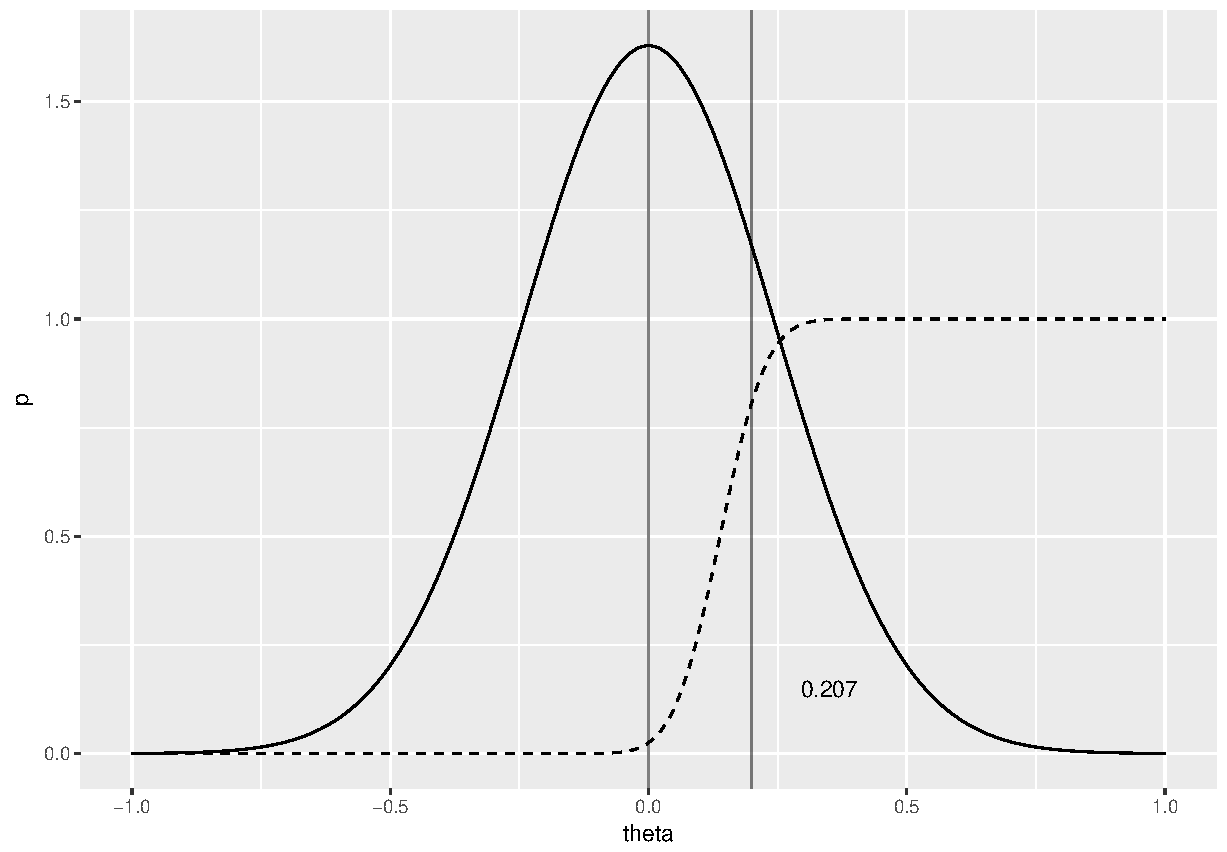
\includegraphics[scale=0.5]{prior_eff}
\end{frame}

\begin{frame}
\frametitle{Example - fixed $\alpha$}
Expected utility for different $n$, all with $\alpha = 0.025$ (one-sided) and \textbf{MCID = 0.2}:

\centering
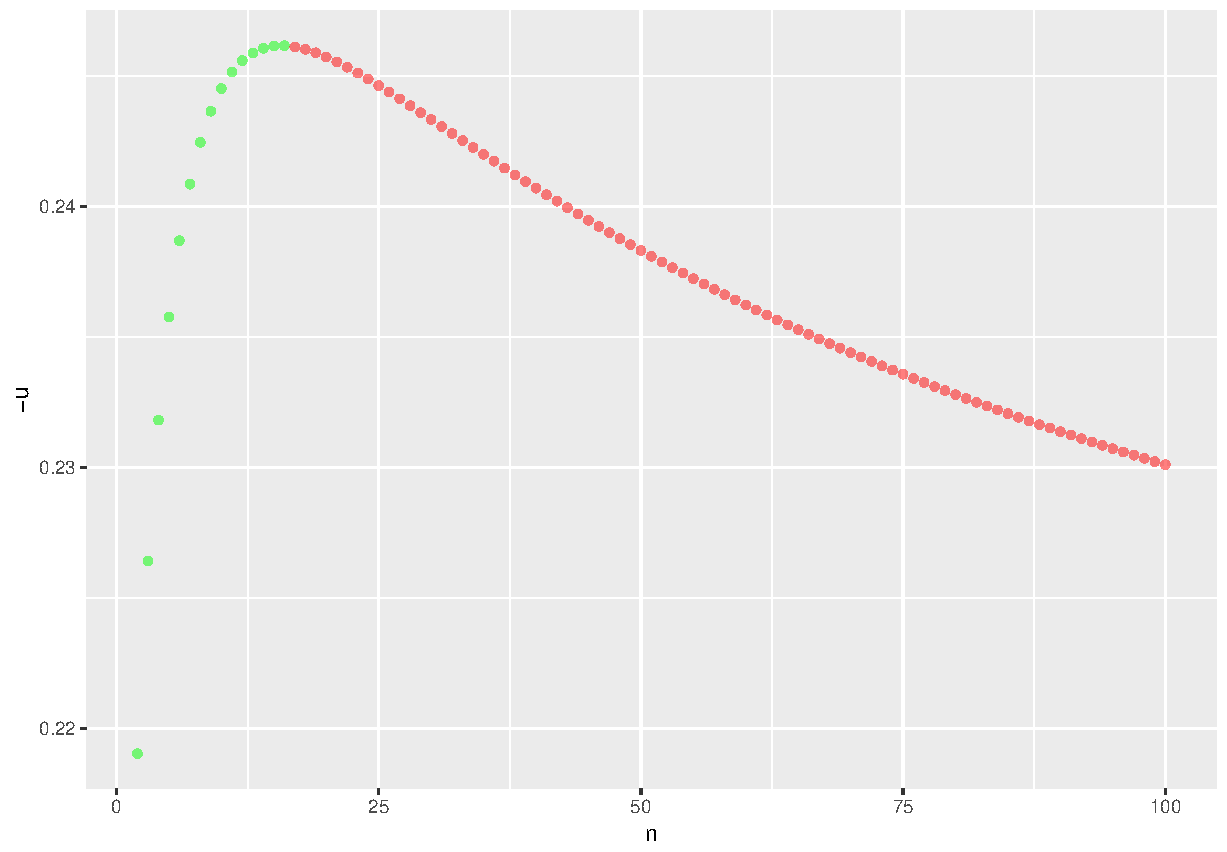
\includegraphics[scale=0.4]{fix_a_2}

Maximum utility at $n = 16$.
\end{frame}


\begin{frame}
\frametitle{Example - fixed $\alpha$}
Expected utility for different $n$, all with $\alpha = 0.025$ (one-sided) and \textbf{MCID = 0.05}:

\centering
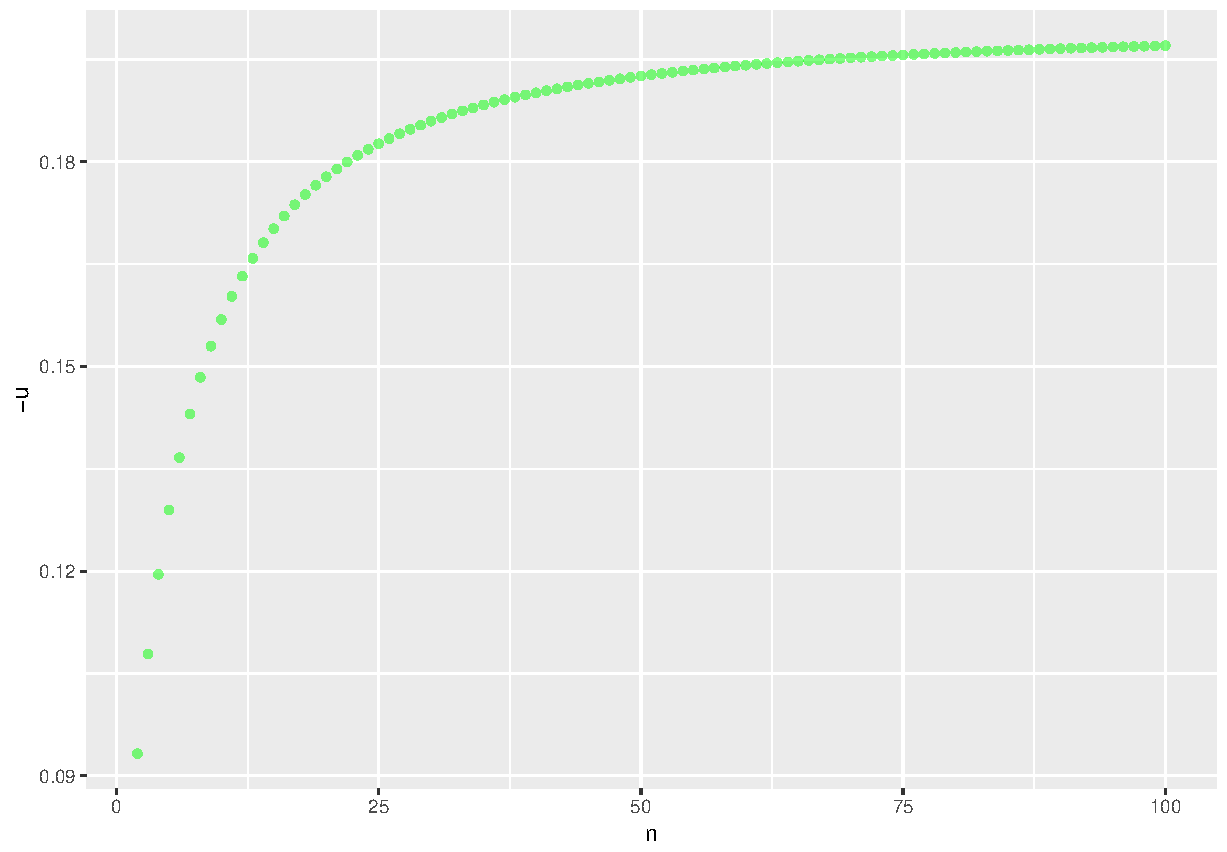
\includegraphics[scale=0.4]{fix_a_05}

Maximum utility at $n > 100 $.
\end{frame}


\begin{frame}
\frametitle{Example - fixed $\alpha$}
Expected utility for different $n$, all with $\alpha = 0.025$ (one-sided) and \textbf{MCID = 0.142}:

\centering
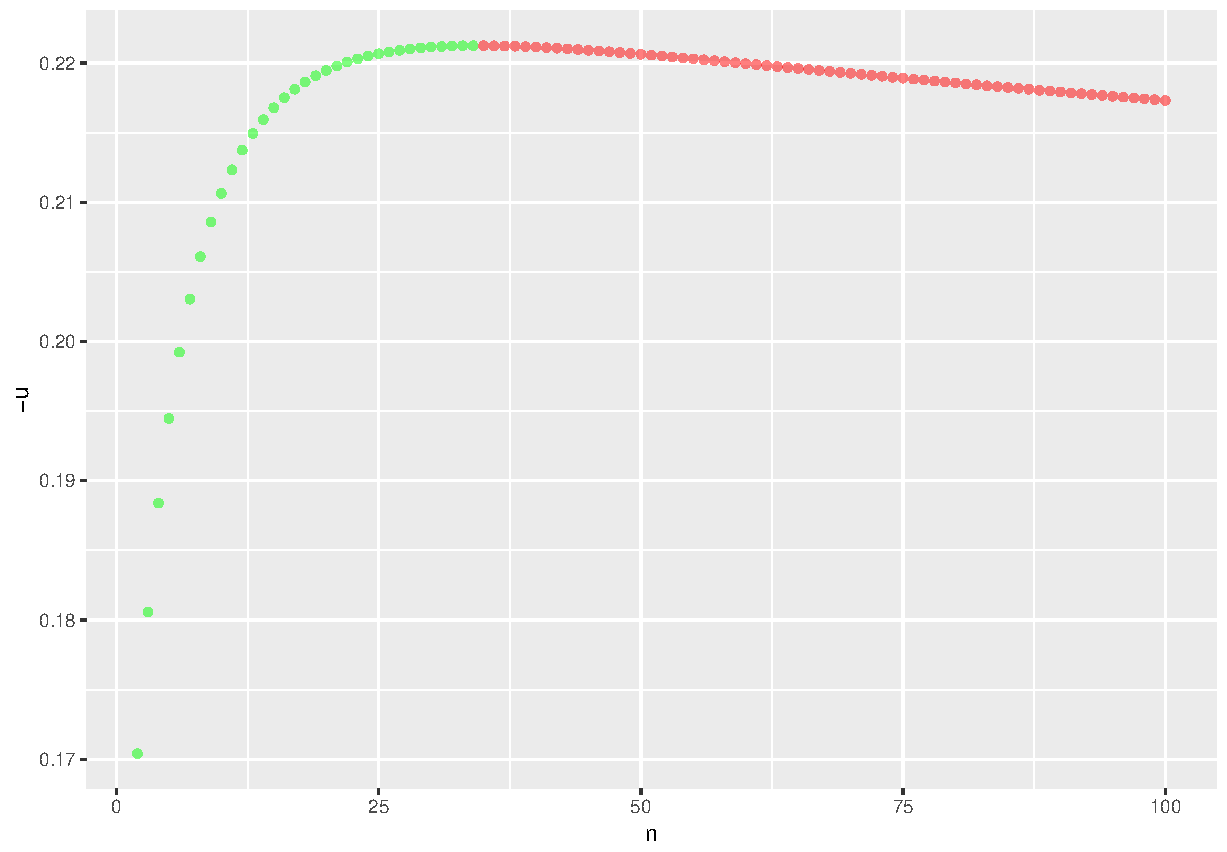
\includegraphics[scale=0.4]{fix_a_142}

Maximum utility at $n = 34 $.
\end{frame}

\begin{frame}
\frametitle{Example - fixed $\alpha$}
Corresponding conditional power at $\theta=0.2$, for \textbf{MCID = 0.142}:

\centering
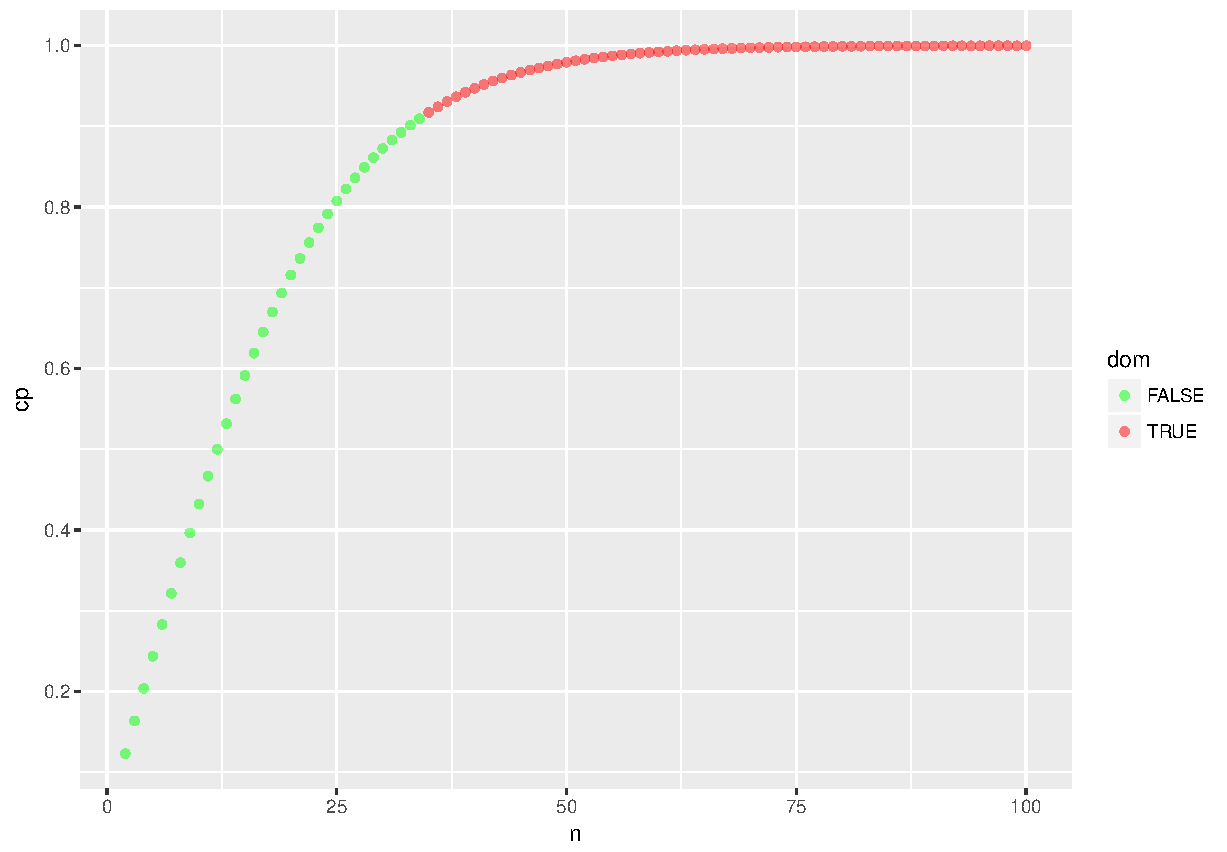
\includegraphics[scale=0.4]{pow_142}

\end{frame}

\begin{frame}
\frametitle{Aside - the MCID}
Cook \emph{et al.}, ``Specifying the target difference in the primary outcome for a randomised controlled trial: guidance for researchers'', \emph{Trials}, 2015.\\
\vspace{3mm}
``\ldots the difference in the primary outcome value that the study is designed to detect \emph{reliably}.'' [my italics]\\
\vspace{3mm}
``the smallest difference \ldots which patients perceive as beneficial and which would mandate, in the absence of troublesome side effects and excessive cost, a change in the patient's management.''\\
\vspace{3mm}
Our definition implies that for $\theta \approx \theta^{*}$, we are indifferent between recommending and rejecting the treatment.
\end{frame}

\begin{frame}
\frametitle{Aside - the MCID}
Why $\theta^{*} = 0.142$?

\begin{itemize}
\item The original design was to give 80\% power at $\theta = 0.2$ for $n = 25$.
\item With the same sample size, we have $\approx 50$\% power at $\theta = 0.142$.
\item Should a frequentist design always have 50\% power at (our) MCID? Is this the point of equipoise? Are MCIDs defined in practice as the effect we want to detect with 80\% power? And if so, can we justify adjusting sample size and power around this MCID?
\end{itemize}
\end{frame}

\begin{frame}
\frametitle{Example - free $\alpha$}
Maximising expected utility over $\alpha$ for each $n$ - \textbf{MCID = 0.2}:

\centering
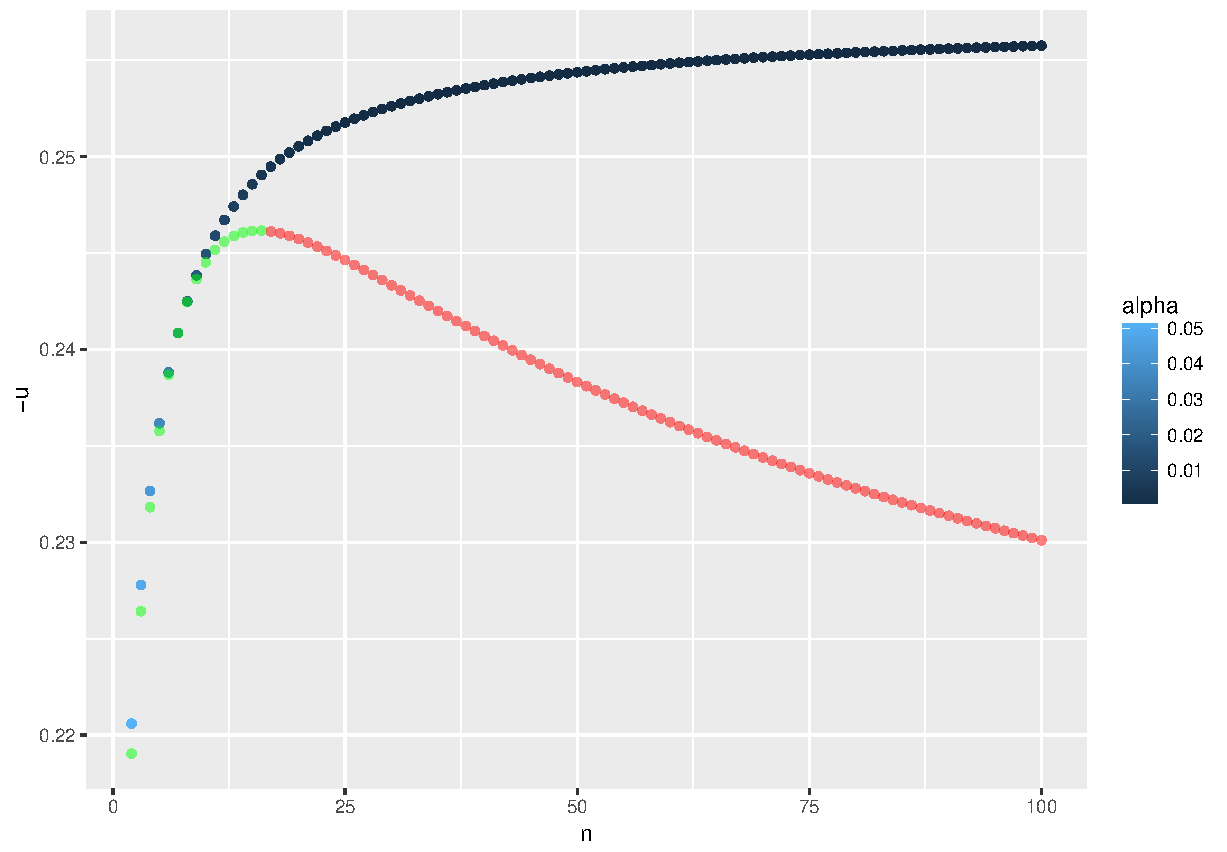
\includegraphics[scale=0.4]{free_a_2}
\end{frame}

\begin{frame}
\frametitle{Example - free $\alpha$}
Maximising expected utility over $\alpha$ for each $n$ - \textbf{MCID = 0.05}:

\centering
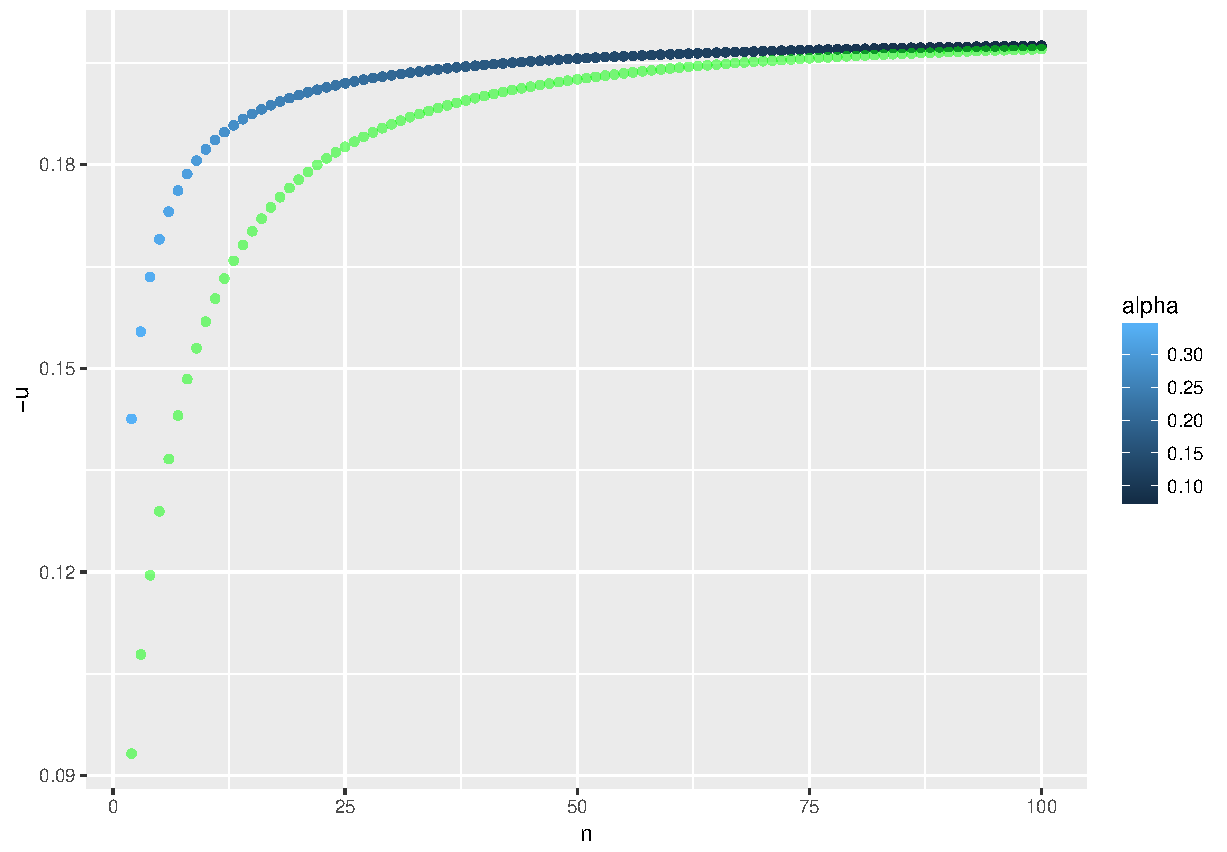
\includegraphics[scale=0.4]{free_a_05}
\end{frame}

\begin{frame}
\frametitle{Example - free $\alpha$}
Maximising expected utility over $\alpha$ for each $n$ - \textbf{MCID = 0.142}:

\centering
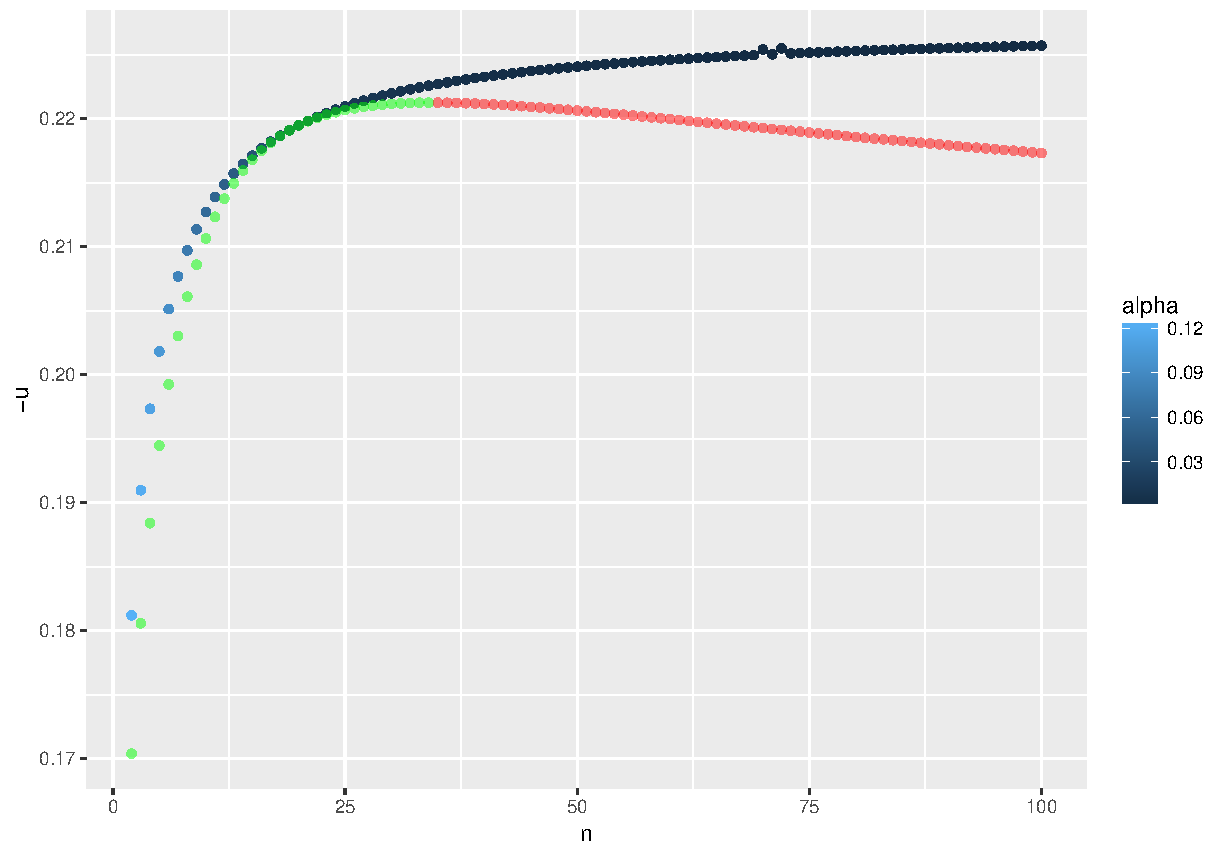
\includegraphics[scale=0.4]{free_a_142}
\end{frame}

\begin{frame}
\frametitle{Example - free $\alpha$}
Operating characteristics (power at $\theta = 0.2$) of these efficient designs:

\centering
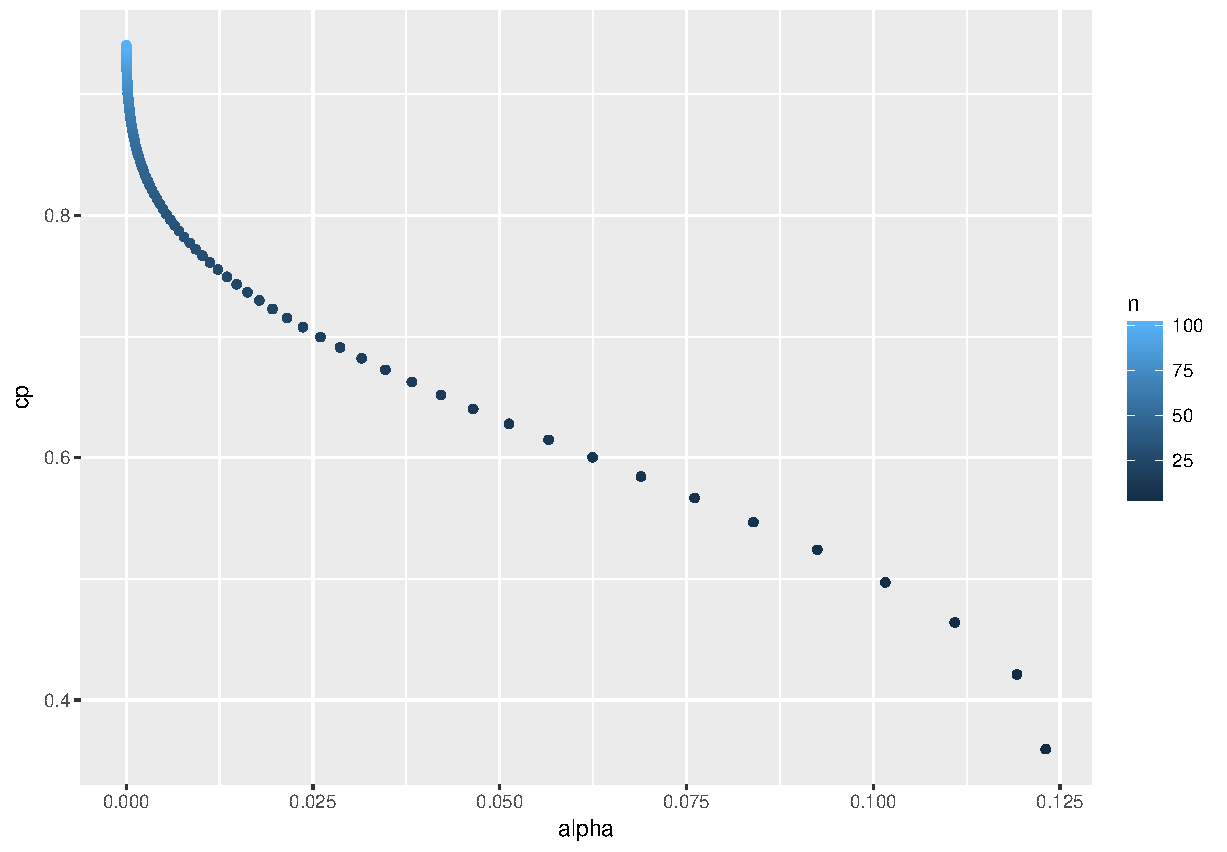
\includegraphics[scale=0.4]{OCs}
\end{frame}

\begin{frame}
\frametitle{Example - free $\alpha$}
Operating characteristics (power at $\theta = 0.2$) of these efficient designs:

\centering
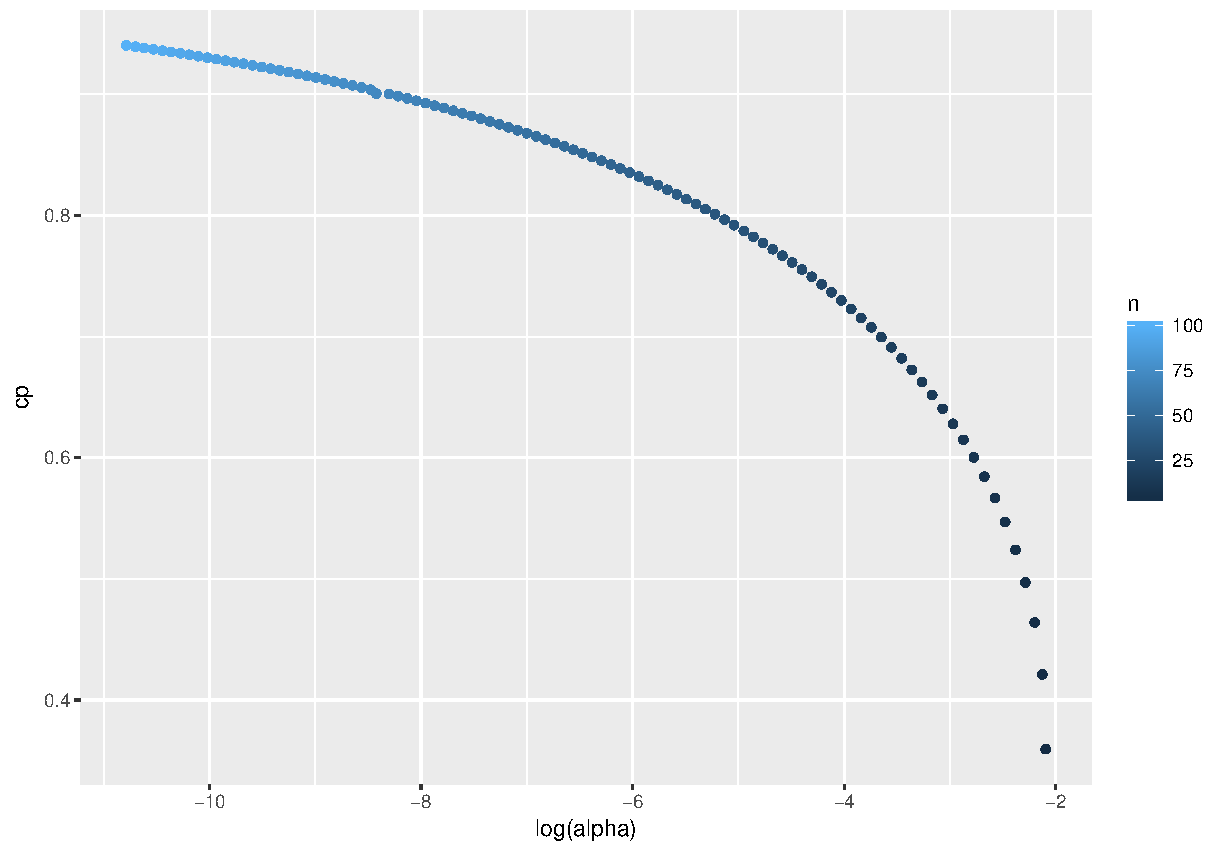
\includegraphics[scale=0.4]{OCs_log}
\end{frame}


\begin{frame}
\frametitle{Critical values}
Each optimal design specifies $n$ and a critical value $c$ to be used in the test. We see that:

\begin{itemize}
\item As $n$ increases, the $c$ approaches $\theta^{*}$ (from above);
\item The optimal design for each $n$ specifies a critical value which, if observed, would give us a posterior distribution on $\theta$ which gives $Pr[\theta > \theta^{*} | \bar{x} = c] = 0.5$.
\end{itemize}

Latter is a consequence of having a symmetric utility and a symmetric posterior distribution on $\theta$.
\end{frame}


\begin{frame}
\frametitle{Non-linear utility}
We transformed a value function into a utility function, but a risk-neutral approach made no difference. Consider the exponential utility:

\begin{equation}
  u(c) =
    \begin{cases}
      (1 - e^{-ac})/a & \text{if } a \neq 0\\
      c & \text{if } a = 0
    \end{cases}       
\end{equation}

\begin{itemize}
\item $ a > 0 \Rightarrow $ risk \emph{averse};
\item $ a < 0 \Rightarrow $ risk \emph{seeking}.
\end{itemize}

Uniquely, implies \emph{constant absolute risk aversion}.
\end{frame}


\begin{frame}
\frametitle{Non-linear utility}
\centering
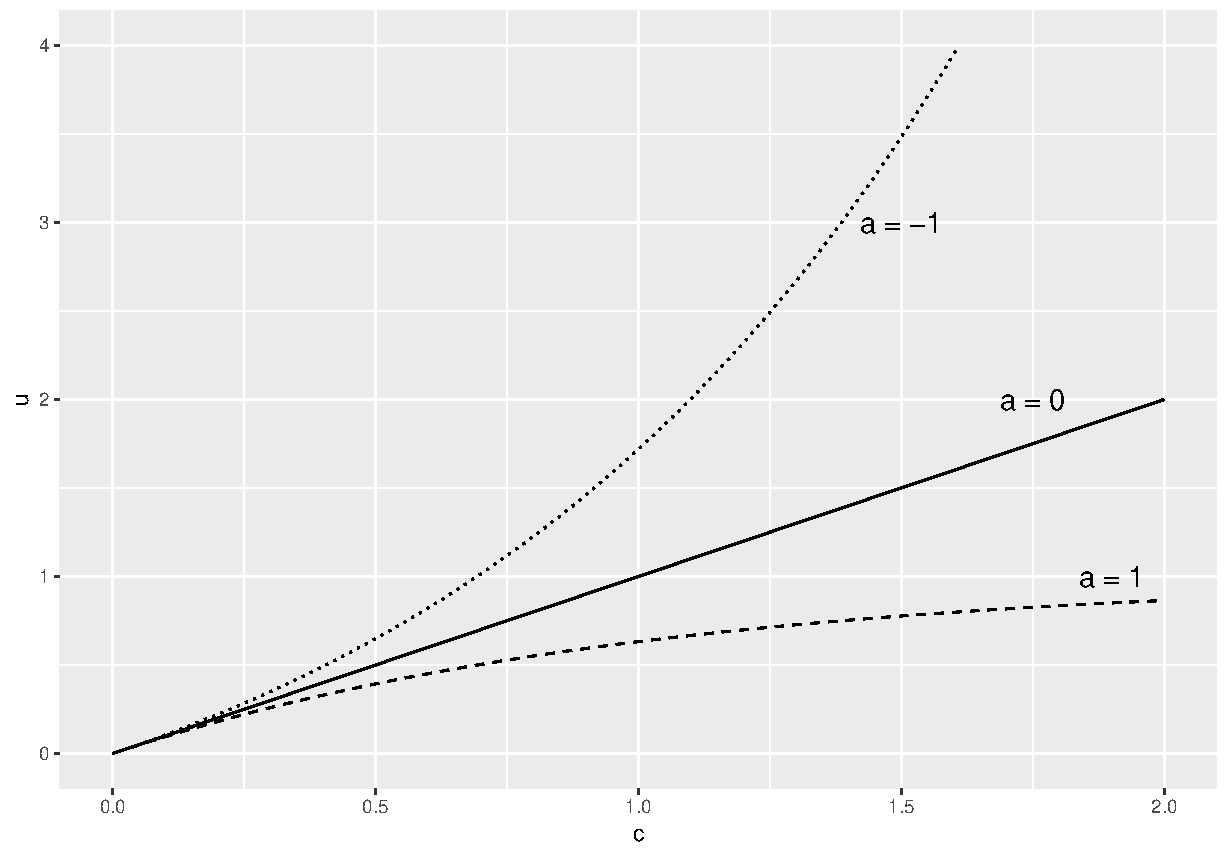
\includegraphics[scale=0.5]{exp_u}
\end{frame}


\begin{frame}
\frametitle{Multi-attribute utility}
Recall that we assumed $\theta$ and $n$ were preferentially independent. If we further assume that out attitude to risk on each attribute doesn't depend on the other, we have an additive utility function:
\begin{equation}
u(\theta, n) = u_{1}(\theta) + ku_{2}(n).
\end{equation}
Given the individual utilities $u_{1}, u_{2}$ we can determine $k$ by asking for the $\theta$ such that
\begin{equation}
(\theta, n_{*}) \sim (\theta_{*}, n^{*})
\end{equation}
\end{frame}

\begin{frame}
\frametitle{Multiple nuisance parameters}
\textbf{What has all this got to do with pilot trials??}

\begin{itemize}
\item Provides a simple way to use all information (recruitment, follow-up, variability, efficacy, safety, adherence \ldots);
\item Allows for trade-offs between intervention attributes;
\item Models the link between the pilot and main study, allowing for optimal pilot design.
\end{itemize}

\end{frame}

\begin{frame}
\frametitle{Joint pilot/confirmatory design}
Using the same example but with $\sigma = 1$:\\\vspace{5mm}
\begin{tabular}{llllllll}
\toprule
\multicolumn{3}{c}{Pilot} & \multicolumn{3}{c}{Confirmatory} & & \\
$\alpha_{1}$ & $\beta_{1}$ & $n_{1}$ & $\alpha_{2}$ & $\beta_{2}$ & $n_{2}$ & $\mathbb{E}[n]$ & $\mathbb{E}[u]$   \\
\midrule
0.41 & 0.97 & 209 & 0.0001 & 0.90 & 1227 & 781.3 & 0.393 \\
0.43 & 0.94 & 150 & 0.018 & 0.77 & 408 & 341.1 & 0.391 \\
0.43 & 0.78 & 43 & 0.121 & 0.65 & 119 & 98 & 0.380 \\
\bottomrule
\end{tabular}
\end{frame}

\begin{frame}
\frametitle{Nuisance parameters}
Nuisance parameters are those which will influence the power of the confirmatory trial, but otherwise are not in the utility function. Recall,

\begin{equation}
\mathbb{E}_{\mathbf{\theta}}[u(d, \mathbf{\theta})] = \int \{g(d, \mathbf{\theta})(\theta - \theta^{*}) + [1- g(d, \mathbf{\theta})](\theta^{*} - \theta)\}p(\mathbf{\theta}) d\mathbf{\theta}.
\end{equation}

\begin{itemize}
\item Now a multi-dimensional integration over vector $\theta$;
\item Not analytically tractable $\rightarrow$ Monte Carlo approximation;
\item Can use samples from the MCMC analysis of pilot data (for every design evaluated);
\item Challenges when analytic expression for $g(d, \theta)$ unavailable.
\end{itemize}

\end{frame}


\end{document}
